\documentclass[aspectratio=169]{beamer}
%\usetheme{CambridgeUS}
%\usecolortheme{beaver}

%\usefonttheme{serif}
%\usepackage{helvet}

\usefonttheme{serif}     % Font theme: serif
%\usepackage{ccfonts}     % Font family: Concrete Math
\usepackage[T1]{fontenc} % Font encoding: T1

\setbeamersize{text margin left=42pt,text margin right=42pt} 
\setbeamertemplate{navigation symbols}{}
\setbeamertemplate{itemize items}[default]

\beamertemplatenavigationsymbolsempty

\definecolor{fore}{RGB}{51,51,51}
\definecolor{back}{RGB}{255, 254, 250}
\definecolor{title}{RGB}{ 255, 15, 0}
\definecolor{links}{RGB}{18, 168, 255}

\setbeamercolor{titlelike}{fg=title}
\setbeamercolor{normal text}{fg=fore,bg=back}
\setbeamercolor{alerted text}{fg=title}
\setbeamercolor{itemize item}{fg=title}
\setbeamercolor{enumerate item}{fg=title}
\hypersetup{colorlinks,urlcolor=links}

% for code https://kbroman.org/blog/2013/10/07/better-looking-latexbeamer-slides/
\usepackage{listings}
\definecolor{keywords}{RGB}{255,0,90}
\definecolor{comments}{RGB}{60,179,113}
\lstset{language=Python,
keywordstyle=color{keywords},
commentstyle=color{comments}emph}

% fonts
\usepackage[sc]{mathpazo}


% title info
\title{\textbf{Public Transit:}}
\subtitle{\textbf{GGR424 - Transportation Geography \& Planning}}
\author{Jeff Allen}
\institute{University of Toronto}
\date{January 31, 2022}


\begin{document}
	
\begin{frame}
	\titlepage	
\end{frame}

%
%\begin{frame}
%	
%	\begin{itemize}
%		
%		\item What is public transit?
%		
%	\end{itemize}
%		
%\end{frame}




\begin{frame}
	\begin{columns}
		\begin{column}{0.5\textwidth}
			
			\textbf{What is public transit?}
			
			\small
			
			\begin{itemize}
				\item Regularly scheduled vehicle trips
				\item Open to all paying passengers
				\item Can carry multiple passengers
				\item Whose trips may have different origins, destinations, and purposes
			\end{itemize}
		
			\vspace{2mm}
		
			"transit is about multiple people riding in one vehicle even though they are not intentionally travelling together or even going to the same places"
			
			\vspace{2mm}
			
			Walker (2011)
			
		\end{column}
		
		\begin{column}{0.5\textwidth}
			\begin{figure}
				\centering
				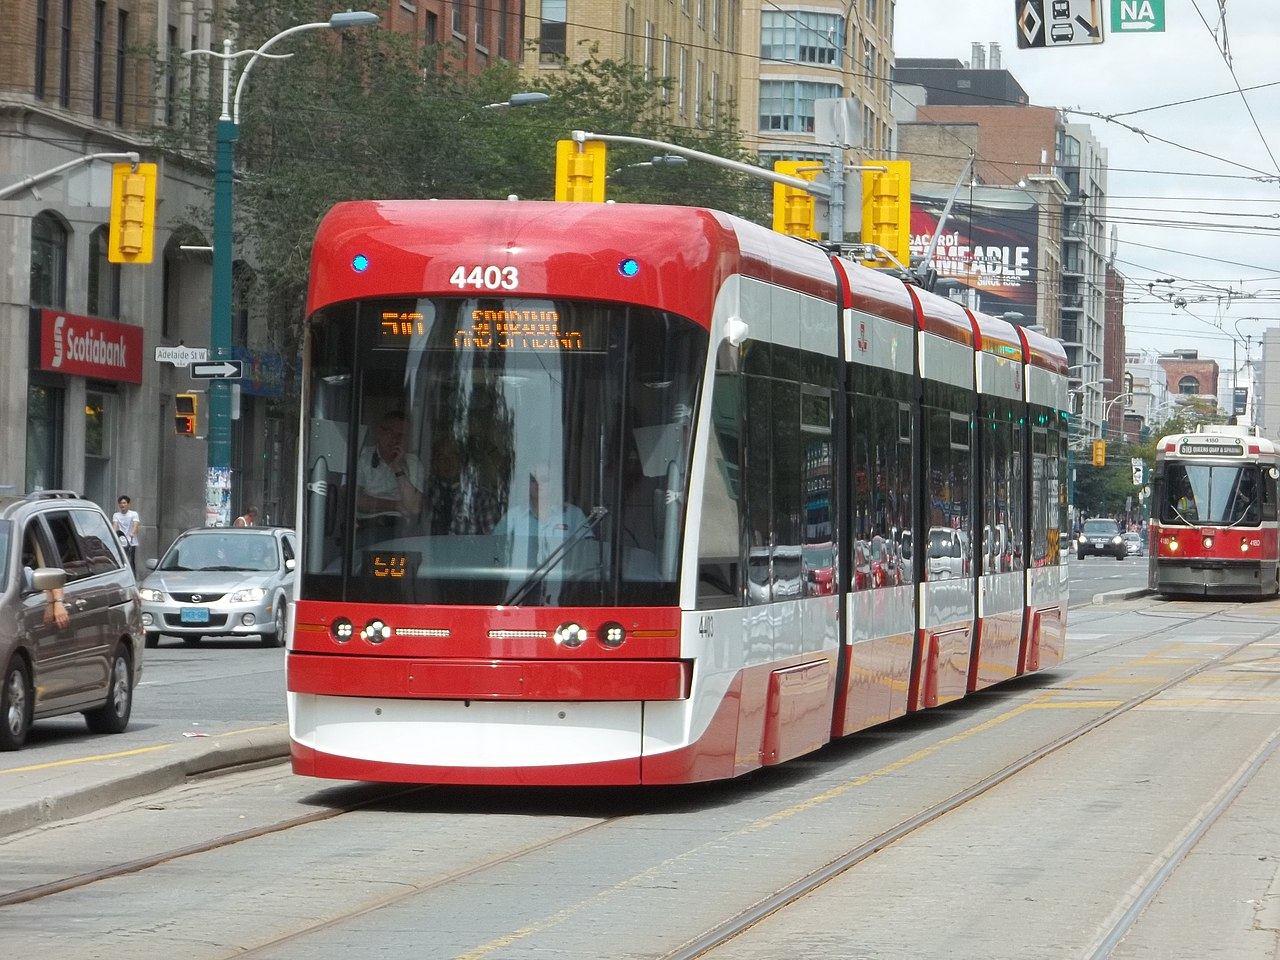
\includegraphics[width=1\linewidth]{images/spadina_streetcar.jpg}
			\end{figure}
			
		\end{column}
		
	\end{columns}
\end{frame}





\begin{frame}
	
	\textbf{Public Transit Benefits}: Efficiency
	
	\begin{figure}
		\centering
		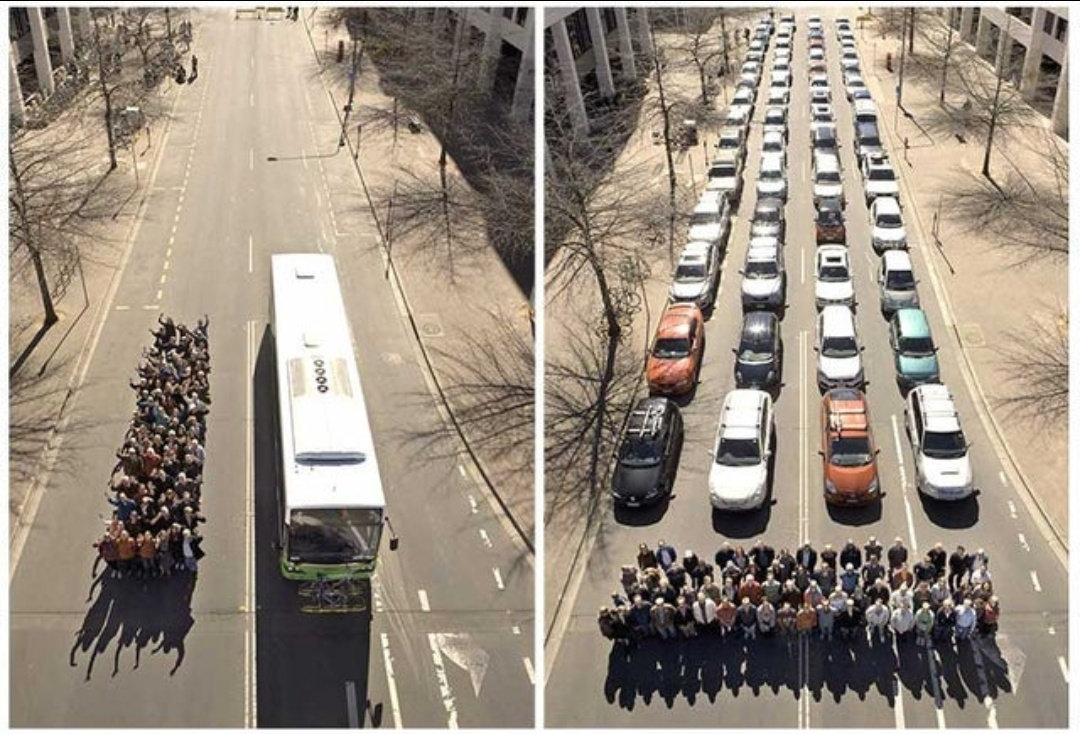
\includegraphics[width=0.8\linewidth]{images/transit_vs_car.jpg}
	\end{figure}

	\tiny\url{https://www.reddit.com/r/Damnthatsinteresting/comments/daugu5/public_transport_vs_private_transport/}
	
\end{frame}




\begin{frame}

	\textbf{What makes transit useful?} Seven demands of public transit:
	
	\vspace{2mm}
	
	\small
	\begin{enumerate}
		\item It takes me \textit{where} I want to go
		\item It takes me \textit{when} I want to go
		\item It is a good use of my \textit{time}
		\item It is a good use of my \textit{money}
		\item It \textit{respects} me in the level of safety, comfort, and amenity it provides
		\item I can \textit{trust} it
		\item It gives me \textit{freedom} to change my plans
	\end{enumerate}

	\vspace{2mm}
	
	Walker (2011)

\end{frame}


\begin{frame}
	
	
	
	\begin{columns}
		\begin{column}{0.5\textwidth}
			
			Components of a public transit system:
			
			\begin{itemize}
				\item \textbf{Network} - the combination of all connecting routes and stops
				
				\item \textbf{Routes} - connections between stops, usually fixed
				
				\item \textbf{Vehicles} - that traverse routes on set schedules
				
				\item \textbf{Stops} - where people access and exit the network, or transfer between routes
				
			\end{itemize}
			
			
		\end{column}
		
		\begin{column}{0.5\textwidth}
			\begin{figure}
				\centering
				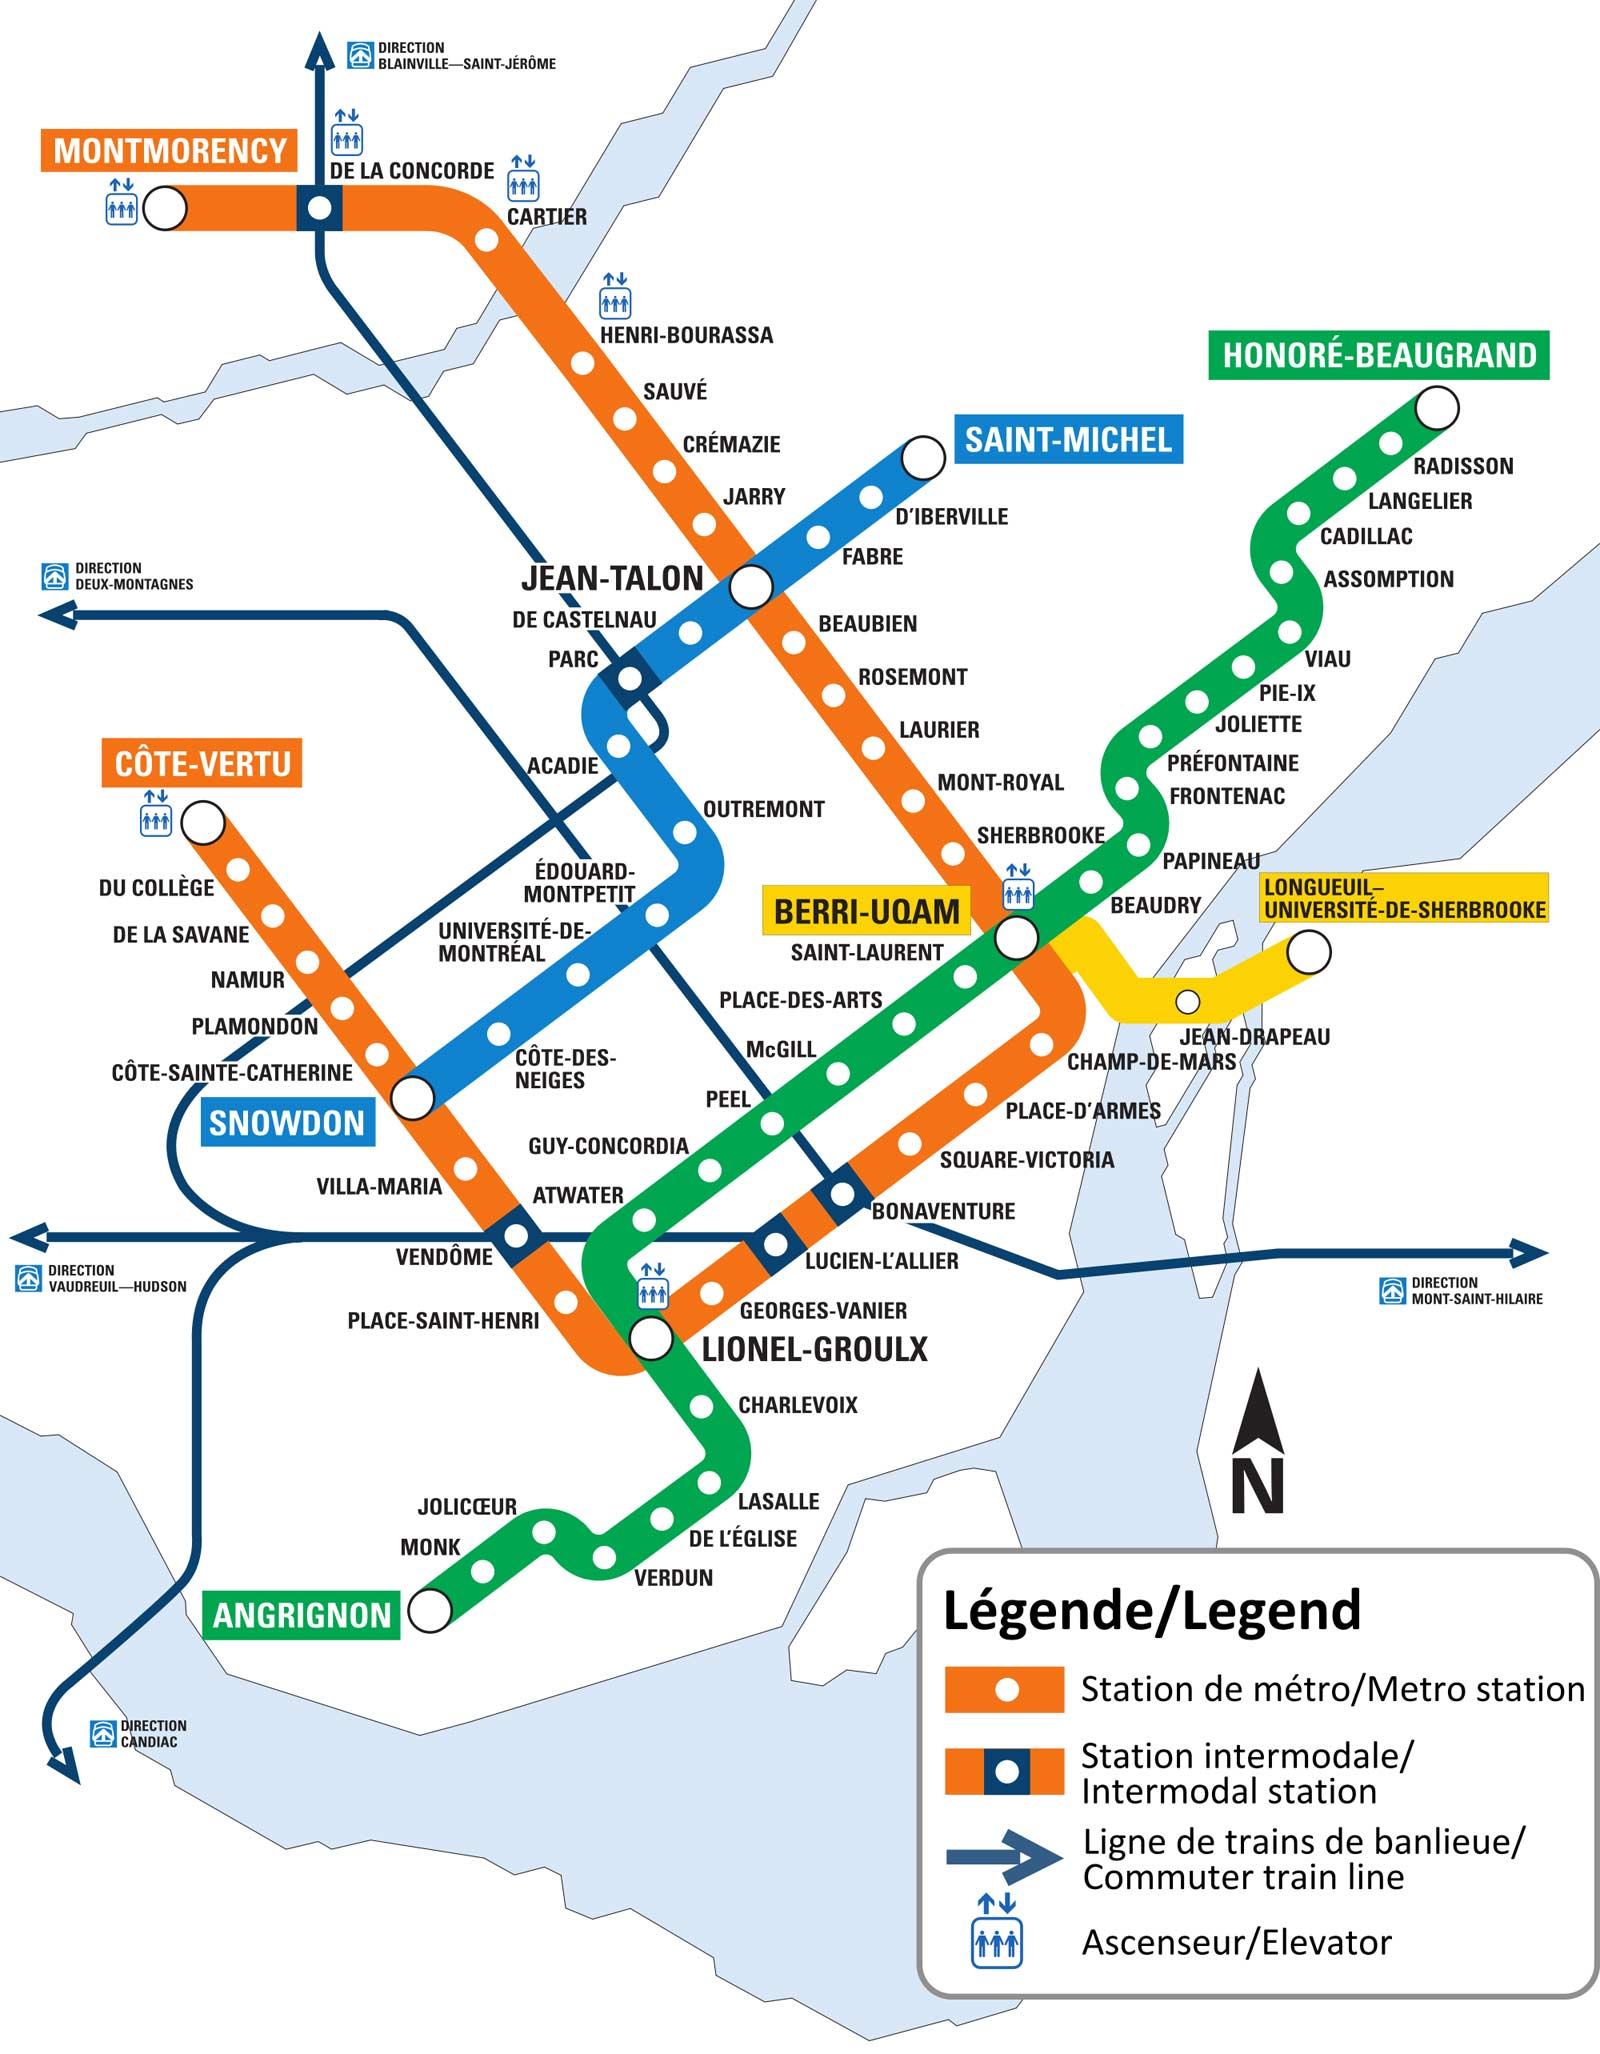
\includegraphics[width=1\linewidth]{images/montreal-metro-map.jpg}
			\end{figure}
			
		\end{column}
		
	\end{columns}
	
\end{frame}




\begin{frame}
	
	Types of transit network layouts: \textbf{Radial}
	
	\begin{figure}
		\centering
		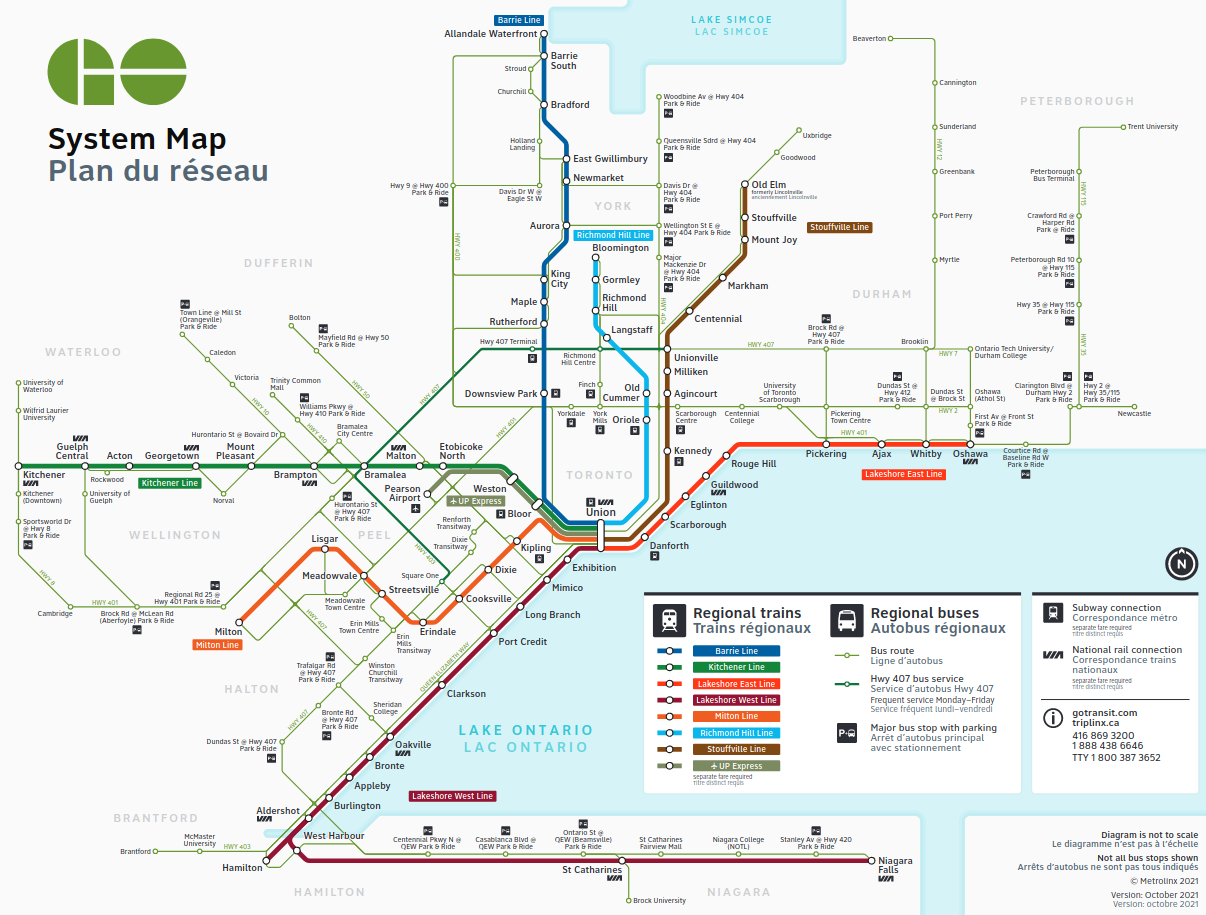
\includegraphics[width=0.7\linewidth]{images/go_map.png}
	\end{figure}

	\tiny\url{https://www.gotransit.com/en/trip-planning/system-and-route-map}
	
\end{frame}



\begin{frame}
	
	Types of transit network layouts: \textbf{Grid}
	
	\begin{figure}
		\centering
		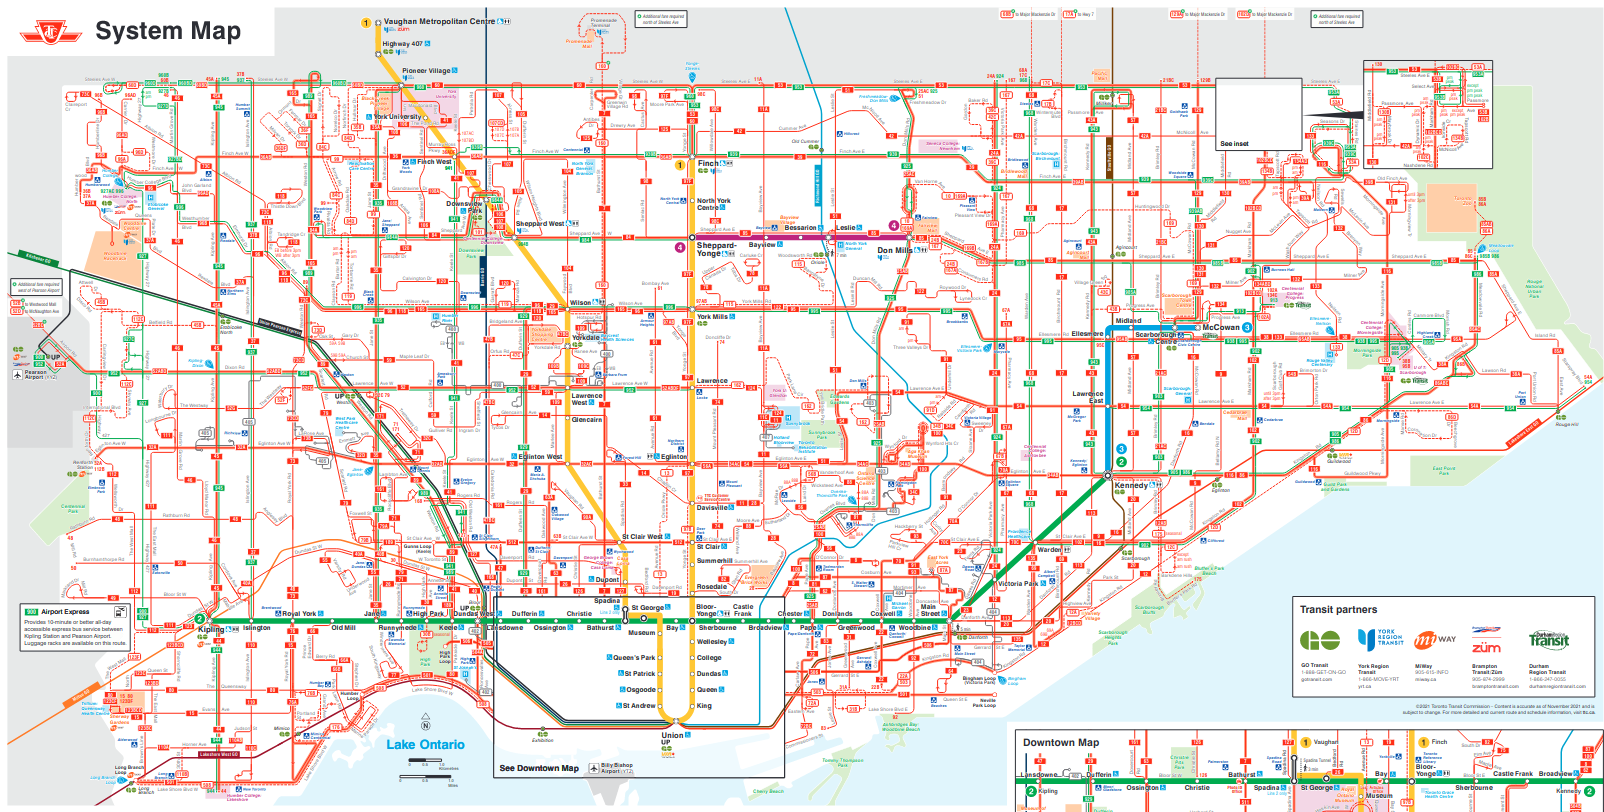
\includegraphics[width=1\linewidth]{images/ttc-map.png}
	\end{figure}

	\tiny\url{https://www.ttc.ca/routes-and-schedules/}
	
\end{frame}


\begin{frame}
	
	Types of transit network layouts: \textbf{Combination}
	
	\begin{figure}
		\centering
		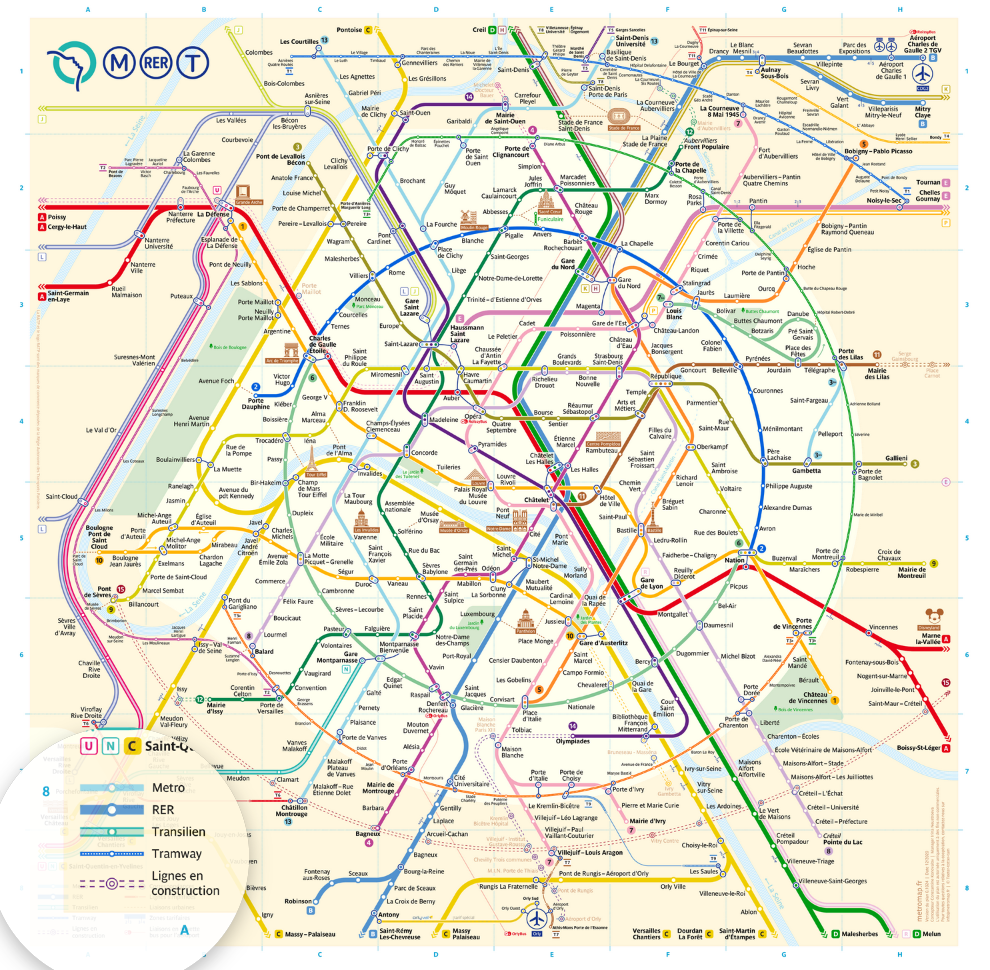
\includegraphics[width=0.6\linewidth]{images/paris_metro.png}
	\end{figure}
	
	
	\tiny \url{https://metromap.fr/en}
\end{frame}



\begin{frame}
	
	\textbf{Routes Characteristics:
	}
	
	\vspace{2mm}
	\begin{itemize}
		\item Technology
		\item Level of separation from other transport
		\item Speed
		\item Capacity
		\item Frequency
		\item Stop Spacing
	\end{itemize}
	
\end{frame}


\begin{frame}
	
	\textbf{Routes} - Technology 
	
\end{frame}


\begin{frame}
	
	\textbf{Routes} - Regional 
	
\end{frame}



\begin{frame}
	
	\textbf{Routes} - Intra-urban Rapid Transit 
	
\end{frame}



\begin{frame}
	
	\textbf{Routes} - LRT / BRT
	
\end{frame}



\begin{frame}
	
	\textbf{Routes} - Surface Routes
	
\end{frame}



\begin{frame}
	
	\textbf{Routes} - Frequency
	
\end{frame}



\end{document}